%----------------------------------------------------------------------------------------
%	PREPROCESSING PIPELINE AND DATA SET CREATION
%----------------------------------------------------------------------------------------
\section{Preprocessing and data set creation}
\label{ch:Dataset}

In this chapter, the different preparatory steps for the recorded data are described, including the creation of a data set which is usable for any machine learning or computer vision approach to analyze the image data.

In~\ref{sec:Preprocessing}~\nameref{sec:Preprocessing} the data is assessed and simplified for any further processing. The second section,~\ref{sec:AutomaticFeatureExtraction}~\nameref{sec:AutomaticFeatureExtraction}, deals with the creation of feature scripts that were researched and implemented for an automatic recognition of single features.
The results were combined in an application which is described in detail in~\ref{sec:LabelApp}~\nameref{sec:LabelApp}. In~\ref{sec:ManualLabeling}~\nameref{sec:ManualLabeling}, the process of hand-labeling the images for their features with the label application is described, followed by a section analyzing the results and comparing the overall agreement of the labelers. The last section~\ref{sec:AsparagusDataSet}~\nameref{sec:AsparagusDataSet} concludes with the creation of the final data set, used for the training of the neural networks and other approaches to detect the label of a spear from its three images.

\begin{figure}[!hb]
    \centering
    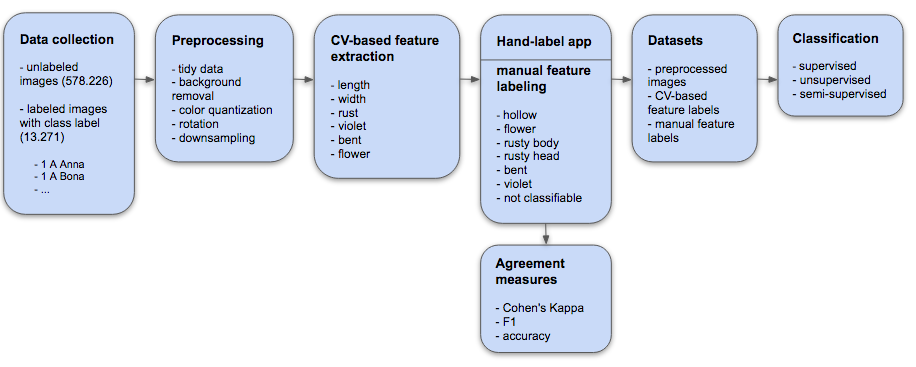
\includegraphics[width=0.98\textwidth]{Figures/chapter03/working_steps.png}
    \decoRule
    \caption[Working Steps from Data Collection to Classification]{\textbf{Working Steps from Data Collection to Classification}~~~Overall, 578226 unlabeled images were collected. Additionally, 13271 images with a class label were collected (see \autoref{tab:LabeledClassNumber} for the number of images per class label). The collected images go through different preprocessing steps. The preprocessed images are then taken as input to the various algorithms implemented in this project. Further, the preprocessed images combined with the computer vision based, extracted features (see \autoref{sec:AutomaticFeatureExtraction}) are taken as input to the hand-label app. With the help of the application, features are manually labeled by seven annotators. Agreement measures are calculated to compare agreement across annotators. The preprocessed images, the computer vision based features, and the manual labels are taken to create different datasets, which are further used for the different classification approaches.}
    \label{fig:WorkingSteps}
\end{figure}


\subsection{Preprocessing}
\label{sec:Preprocessing}

Before implementing any approach, the recorded image data has to go through multiple preprocessing steps.

The goal of this preprocessing is to reduce the variance by removing the background, shifting the asparagus spear to the center of the image patch and rotating it upwards. Correct orientation is especially important to make approaches such as \acrshort{pca} applicable and facilitates direct measuring of features. Background removal facilitates the measurement of features like width and height of the spears, because the position of foreground pixels per column can be easily evaluated (see \autoref{sec:AutomaticFeatureExtraction}).

In the following, the different preprocessing steps are elaborated in detail.\footnote{See \url{https://github.com/CogSciUOS/asparagus/blob/FinalProject/preprocessing/perform\textunderscore preprocessing.py} (as of 11/27/2020)}

\bigskip
As described in~\autoref{sec:DataCollection}, each asparagus is depicted in three pictures, one in each of the three positions \textendash{} left, center and right. The image names are used to find the three relevant images and determine in which position the asparagus is captured. The images are cut into three pieces and renamed in a way that makes clear which images belong together. Each asparagus gets a unique identification number and the three perspectives are denoted with \textit{a} for left, \textit{b} for center, and \textit{c} for right. For example, the \texttt{image 42\textunderscore b.png} is the center image of the asparagus spear with the identification number 42.

Another step is to remove the background of the image. As the conveyor belt is blue, there is a high contrast to the bright asparagus spears which facilitates background removal (see \autoref{fig:PreprocessingCropping}). Hence, it is possible to mask the asparagus spear using the hue of the HSV representation of each image. All pixels with a blue hue and very dark regions are marked as background through threshold limitation of the value component. This is particularly important for the automatic feature extraction (see~\autoref{sec:AutomaticFeatureExtraction}).

\begin{figure}[!ht]
	\centering
	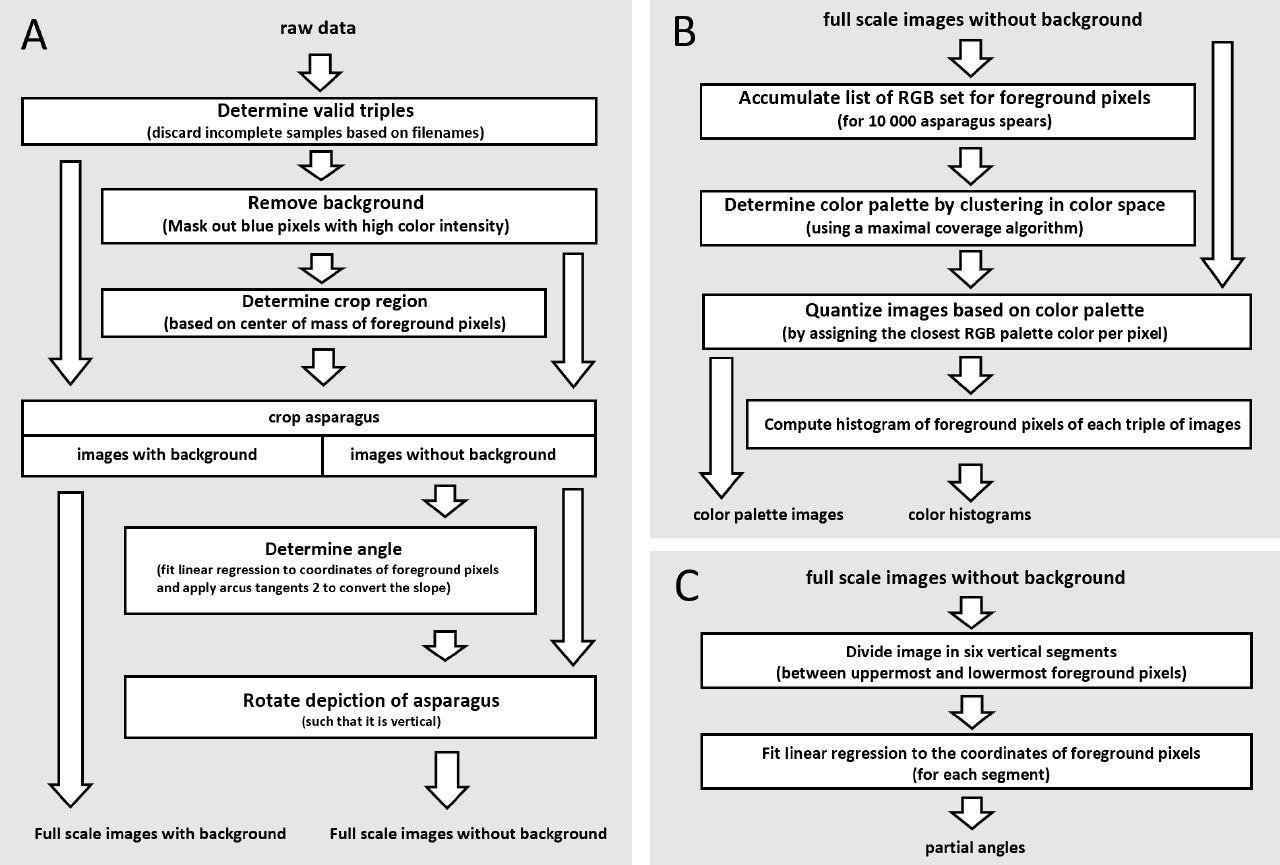
\includegraphics[width=0.98\textwidth]{Figures/chapter03/preprocessing_pipeline.png}
	\decoRule
	\caption[Preprocessing Pipeline]{\textbf{Preprocessing Pipeline}~~~The depiction shows the preprocessing pipeline that was used to generate different datasets. For each asparagus spear three images were saved. Downscaled versions were computed for each image dataset. A: The processing steps to retrieve full-scale images with and without background. B: The approach to retrieve color palette images and color histograms by feature engineering. C: Processing steps for the retrieval of partial angles. For details on B and C see also \autoref{subsec:FeatureEngineering}.}
	\label{fig:PreprocessingPipeline}
\end{figure}

\begin{figure}[!ht]
	\centering
	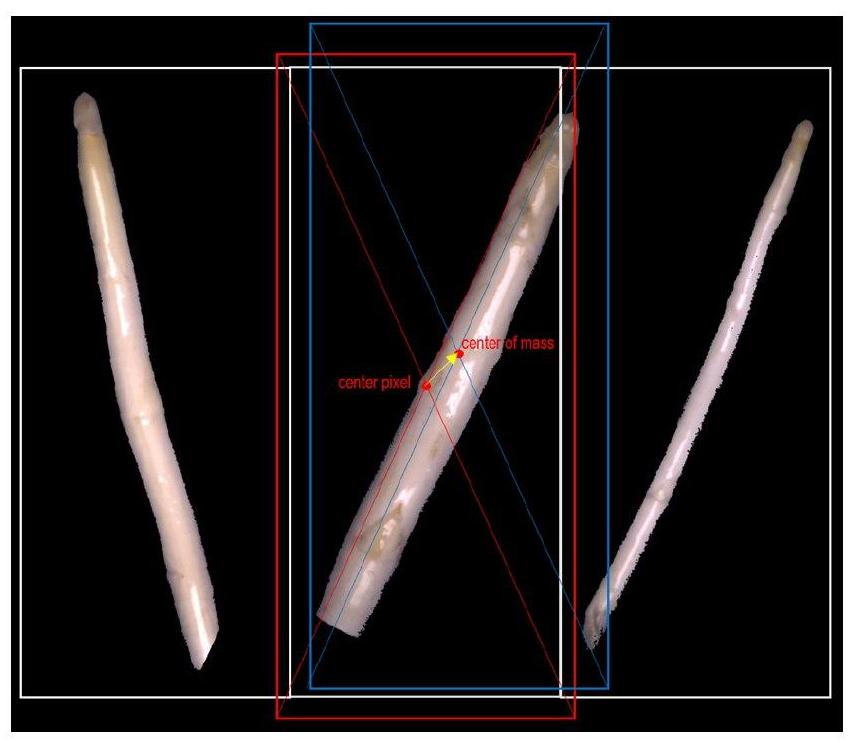
\includegraphics[width=0.95\textwidth]{Figures/chapter03/preprocessing_cropping.png}
	\decoRule
	\caption[Cropping Based on Center of Mass]{\textbf{Cropping Based on Center of Mass}~~~The depiction shows the effect of moving the cropping window (red) to a new location (blue) by moving it's center horizontally towards the center of gravity (yellow arrow). The buckets on the conveyor belt are illustrated by white boxes. The approach is applicable for all three images given that the initial coordinates are set to the respective positions. For unprocessed images see \autoref{fig:ExampleImagesAnna}.}
	\label{fig:PreprocessingCropping}
\end{figure}

\bigskip
Subsequently, each triple of images that depict one piece from different angles is determined and the area that shows the correct piece is cropped. The cropping regions are set to three patches that are a little larger than the compartments of the conveyor belt. They are located such that they cover the spear of interest which can either be at the left, center or right (see \autoref{fig:ExampleImagesAnna}). As it has been found that some tilted spears span across the borders between the conveyor compartments, the cropping window in the images was moved. The new coordinates are determined by shifting the center of the current cropping box horizontally to the center of mass of the contained foreground pixels (see \autoref{fig:PreprocessingCropping}). Repeating the procedure in a second iteration can further improve the result. As this is the only case for a small number of examples we refrained from doing so to increase processing speed. Small parts of the neighboring depiction potentially end up in the region of interest as well. These remainders are removed by masking out all pixels that do not belong to the main blob of connected pixels.

\bigskip
To further reduce the variance the asparagus spears are rotated upwards to reduce the variance in angle. The rotation angle is achieved by binarizing the image into foreground and background pixels, calculating the centerline as the mean pixel location along the vertical axis, and fitting linear regression to the centerline pixels.

\bigskip
Another preprocessing step, which generates an additional set of images, is quantization using a common color palette. It was mainly employed to allow for the computation of meaningful color histograms.\footnote{The number of colors in the original 24 bit RGB colorspace is too large to use them as bins for the histograms: The low number of pixels per bin would not allow for meaningful statistics. By reducing the number of colors the problem is solved.} An appropriate palette and the respective mapping of RGB values to palette colors is determined using clustering in color space. First, a set of RGB tuples is collected by adding pixel values of 10000 asparagus spears. Second, the resulting list of RGB tuples is converted to an image such that a palette can be determined using standard tools for quantization. In the last step, a clustering algorithm is employed that determines the position of cluster centers while maximizing the maximal coverage. The resulting cluster centers can be displayed as a list of RGB values which represent the color palette.\footnote{Here we used a standard implementation for image quantization that employs a maximal coverage algorithm ~\citep{pil_quantization}. An optimal solution to the problem of maximum coverage relates to the challenge of distributing a given number of circular areas named facilities such that they cover the largest possible area of the sample space ~\citep{zarandi2011large}. One can interpret the centers of named facilities as cluster centers. For each data point (here: pixel), the closest cluster center is determined and the respective value attributed. This means the data is quantized.} The color palette is used for quantization of the images: Each image of the downscaled data set is transformed to the palette representation. Visual inspection shows little quality loss such that it can be assumed that the relevant information for image classification is well preserved.

\bigskip
Several additional collections of preprocessed images are computed based on the data without background. This holds for downscaled versions as well as for a version that contains the asparagus heads only. To compute the latter, the images are padded to avoid sampling outside of the valid image boundaries and the uppermost foreground row is detected. Subsequently, the center pixel is determined and the image is cropped such that this uppermost central pixel of the asparagus is the center of the uppermost row of the snippet. The resulting partial images of asparagus heads are rotated using the centerline regression approach described above. The approach has proven reliable and the resulting depictions are used to train a dedicated network for head related features (see~\autoref{subsec:HeadNetwork}).

\newpage

\subsection{Feature extraction}
\label{sec:AutomaticFeatureExtraction}

The class label of an asparagus spear is decided by several features, ranging from its shape to its color. Put together, these single features give the class label that attributes an asparagus to a quality class (for a description of the quality classes, see \autoref{tab:AsparagusLabels}, and further \autoref{fig:LabelTree} on how features lead to the class label).

\bigskip
We decided to label the images for their features rather than final class labels. The main reason for this was to make the labeling process easier for the inexperienced annotator. The boundaries between class labels are not always clear and can be difficult to detect from image data. Deciding whether a single feature is present or absent in an asparagus spear is more straightforward. Further, the training for the hand labeling and communication about special cases is facilitated. Another reason to label features rather than class labels was to break down the classification problem into smaller problems. Additionally, it is possible to detect which features are more difficult to learn than others, which provides meaningful insight into the classification task. Last but not least, deciding on the class labels after the features are detected reliably is a small step and can be easily done with a decision tree or rule-based approach.

Even though the chosen features closely resemble the class labels defined by Gut Holsterfeld, they are different and should not be confused with one another. The 6 features we labeled by hand are as follows: hollow, flower, rusty body, rusty head, bent and violet. Additionally, the length and width was automatically detected as described below and used to set supplementary labels for very thick, medium thick, thick, thin, very thin, and fractured. Further, images that could not be classified thoroughly were labeled as \enquote{not classifiable} (e.g.\ when the spear is cut off the image).

\bigskip
In this chapter, the different features as well as their extraction methods will be described. The results that are achieved by computationally extracting the features are reported alongside future steps that could be taken to improve the results further. For each feature detection method, the images with removed background are used as displayed in a respective example image shown per feature. Additionally, it is described which features were hand labeled by us. The feature functions, that provide reliable predictions, were integrated into an application, which is described in the subsequent \autoref{sec:LabelApp}, with which human annotators could manually label the unlabeled data.


\subsubsection{Length}
\label{subsec:Length}

The length detection described in the following paragraph was later used to automatically calculate the presence of the feature fractured in an image. An asparagus spear includes the feature fractured if it is broken or if it does in any other way not fulfill the required, minimal length of 210 mm (see \autoref{fig:ExampleFractured}). 

\bigskip
The length detection uses a pixel-based approach. It counts the number of rows from the highest to the lowest pixel that is not a black background pixel and therefore not zero. The asparagus is rotated upwards, as described in~\autoref{sec:Preprocessing}. This is done to improve the results, as the rows between the highest and the lowest pixel are counted and not the pixels themselves. This technique is a simplification, which does not represent curved asparagus accurately, because it will have a shorter count than it would have if the pixels were counted along the asparagus spear.

\begin{wrapfigure}{!I}{0.35\textwidth}
  \begin{center}
    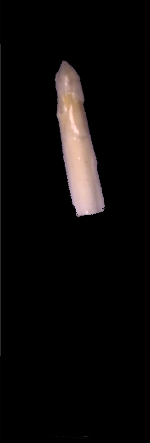
\includegraphics[width=0.15\textwidth]{Figures/chapter03/example_img_fractured.png}
  \end{center}
  \vspace{-15pt}
  \caption[Example Image Feature Fractured]{ \textbf{Feature Fractured}}
  \label{fig:ExampleFractured}
\end{wrapfigure}

However in reality, there are not a lot of asparagus spears close to the decision boundary between a fractured spear and a whole spear. Usually, the asparagus is harvested a few centimeters longer than necessary and then cut to the desired length. The only asparagus shorter than that length are the ones that break during the sorting process. Moreover, if they break, they generally break closer to the center of the asparagus rather than at the ends. Therefore, the difference in length detection does not matter for our purposes.

\bigskip
All in all, by visual inspection the length detection yields good results that are very helpful for the hand-label app. The next step would be to train a decision boundary that determines which number of pixels should be the threshold to differentiate between fractured and not fractured. At first, we tried to calculate this threshold by finding a conversion factor from pixel to millimeter, as we know the cut off in millimeters. But this approach appeared to be more difficult than anticipated, because the conversion factor varies in the different image positions. This problem only became apparent after the asparagus season had ended, for which reason we could not reproduce the camera calibrations in retrospective in order to take well-measured images. Accordingly, the threshold needs to be deduced from the data manually or learned with a machine learning approach.

\begin{wrapfigure}{!I}{0.35\textwidth}
  \centering
  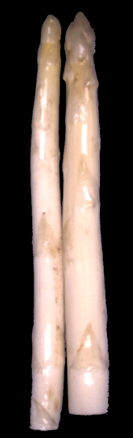
\includegraphics[width=0.15\textwidth]{Figures/chapter03/example_img_thick.png}
  \caption[Example Image Not Classifiable]{ \textbf{Feature Not Classifiable} \\ Example image for the feature not classifiable. Further, a difference in width of both asparagus is observable but the exact thickness is hard to determine by view alone.}
  \label{fig:ExampleThickness}
  \vspace{-15pt}
\end{wrapfigure}

\subsubsection{Width}
\label{subsec:Width}

Like the length of a spear, thickness is a feature that is hardly recognizable by view alone (see for example \autoref{fig:ExampleThickness}). Fortunately, it can also be automatically extracted with a classical approach described in the following section.

\bigskip
The division into different ranges of width can be inferred by the overall thickness of the spear. The feature ‘very thick’ is attributed to asparagus that is more than 26 mm in width. The feature ‘thick’ corresponds to 20 -- 26 mm, the feature ‘medium thick’ to 18 -- 20 mm, and the feature ‘thin’ to 16 -- 18 mm. Every asparagus with less than 16 mm in width is described with the feature ‘very thin’.

\bigskip
The width detection uses a very similar approach as the length detection. It takes the pixel count from the left-most to the right-most pixel in a certain row as a width measure. But in contrast to the length, the width is measured at several image rows from which the mean width is taken. Since the width detection works reliably, it is integrated in the hand-label app (see \autoref{sec:LabelApp}).

The algorithm operates as follows: Firstly, the images are binarized into foreground and background, which means setting all pixels that are not zero, and therefore not background, to one. After that, the uppermost foreground pixel is detected and the length is calculated with the length detection function as described above. The length of the asparagus is used to divide it into even parts. This is done by determining a start pixel and dividing the remaining rows that contain foreground pixels by the number of positions one wants to measure at. This way several rows are selected in which the number of foreground pixels is counted. One can interpret each row as a cross-section of the asparagus, therefore the number of foreground pixels is a direct measure for the width. Then, the mean of these counts is calculated and used as the final width value. As the head of the asparagus can be of varying form and does not represent the width of the whole asparagus well, it is excluded from the measure. This is done by selecting a start pixel below the head area instead of naively choosing the uppermost pixel. To be precise, the start pixel is chosen at 200 pixels, which corresponds to roughly 25 mm, below the uppermost pixel in order to bypass the head area with certainty. As described in the section \nameref{subsec:Length}, also the width detection might lead to slightly different outcomes on curved asparagus spears than the true values. Again, this difference is regarded as irrelevant in our case.


\subsubsection{Rust}
\label{subsec:Rust}

\begin{wrapfigure}{!I}{0.35\textwidth}
  \begin{center}
    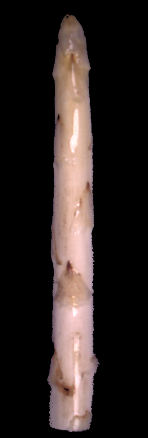
\includegraphics[width=0.15\textwidth]{Figures/chapter03/example_img_rustybody.png}
  \end{center}
  \vspace{-15pt}
  \caption[Example Image Feature Rusty Body]{ \textbf{Feature Rusty Body}}
  \vspace{15pt}
  \label{fig:ExampleRustyBody}
\end{wrapfigure}

The feature rust is split into the sub-features rusty body (see \autoref{fig:ExampleRustyBody}) and rusty head (see \autoref{fig:ExampleRustyHead}). Rust only covering the body can be removed. Whereas rust at the top part of the spear cannot be removed without damaging the head. Thus, rust on the head region is a decisive factor for the quality and later categorization into a price class.

If a spear has rust, it is visible as a dark brown color. It often starts at the tips of becoming leaves or at the bottom part. The color is not to be confused with bruises, pressure marks, or a slightly yellow complexion, which can occur in a ripe asparagus. The latter coloring is neglected.
Rust is set to be present even when only the tip of a leaf shows a dark spot. Other brownish bruises are not classified as rust.

If there is a rusty spot on, or close, to the head region, it is captured by the feature rusty head. The head part is usually distinct in shape and color from the body part of the asparagus. In principle, the same guidelines that apply to the feature rusty body also apply to the feature rusty head, except for an explicit focus on the top part (until around 1 cm below the collar) of the asparagus. Any rust below this is labeled as the feature rusty body.

\begin{wrapfigure}{!I}{0.35\textwidth}
  \begin{center}
    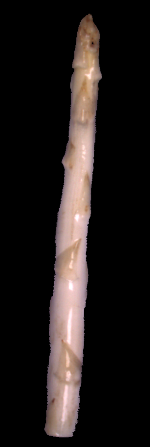
\includegraphics[width=0.15\textwidth]{Figures/chapter03/example_img_rustyhead.png}
  \end{center}
  \vspace{-15pt}
  \caption[Example Image Feature Rusty Head]{ \textbf{Feature Rusty Head}}
  \vspace{-10pt}
  \label{fig:ExampleRustyHead}
\end{wrapfigure}

\bigskip
The automatic rust detection finds all pixels that fall in the range of RGB values that correspond to the color brown. Those pixels are counted and normalized by the maximal number of possible pixels that could be rusty, namely the number of foreground pixels. Since it is impossible that the whole asparagus is rusty and hence that all the foreground pixels fall into the relevant range of RGB values, this normalization yields small numbers as results. To give an example, an output value of 0.13 is already considered moderately rusty. The lower and upper bound for the RGB values are set to $[50,42,30]$ and $[220,220,55]$, respectively. That means, all pixels that have a red value between 50 and 220, a green value between 42 and 220, and a blue value between 30 and 55 are considered to be rust.

\bigskip
Visual inspection shows that the rust detection algorithm works well to detect rusty areas and barely misses any rusty parts. The difficulty lies in setting a threshold for the number of pixels needed to be classified as rusty. Only clusters of brown pixels are reliable indicators for rust.  Many pixels with a brown color distributed over the whole spear are not supposed to be classified as rust. It might be the case that a simple pixel count is not sufficient to set a classification threshold. More sophisticated approaches to detect clusters, such as morphological operators, could be beneficial for this feature detection. It remains unsolved to set a robust threshold that works well on the whole data set.

\bigskip
One problem that cannot be solved algorithmically is dirt in the sorting machine. If the machine is not cleaned thoroughly and regularly, dirt can be falsely classified as rust because it obtains the same color range. Another problem can be a change of illumination when taking the images as a small change in illumination can produce a large change in the appearance of a spear.


\subsubsection{Violet}
\label{subsec:Violet}

The feature violet indicates whether an asparagus is of violet color.
The shift of color from white to violet occurs most often around the head region -- either at the tip of the head or just below the collar of the head region (see \autoref{fig:ExampleViolet}).

As the spear will darken further after it is harvested, even a slightly pink spear is labeled as being violet.

\begin{wrapfigure}{!I}{0.35\textwidth}
  \begin{center}
    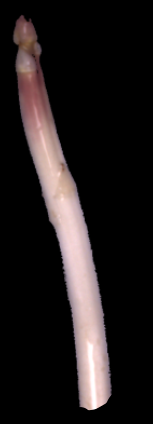
\includegraphics[width=0.15\textwidth]{Figures/chapter03/example_img_violet.png}
  \end{center}
  \vspace{-15pt}
  \caption[Example Image Feature Violet]{ \textbf{Feature Violet}}
  \label{fig:ExampleViolet}
\end{wrapfigure}

\bigskip
According to the UNECE-norm asparagus of the highest quality grade may only be marginally violet or not violet at all ~\citep{unspargelnorm}. Hence it is crucial to sort asparagus pieces according to this binary attribute. In a simple procedure color hues are evaluated. More precisely, this strategy is based on evaluating histograms of color hues that are calculated for foreground pixels of the asparagus images after converting them to the HSV color space. Pale pixels are removed from the selection by thresholding based on the value component of the HSV representation. Finding the optimal threshold has proven difficult because of named subjectivity in color perception. A threshold of 0.3 for the value component is considered a good compromise. All three perspectives are taken into account to compute a single histogram per asparagus spear. A score is calculated by summing up the number of pixels that lie within the violet color range. A second threshold is used as the decision boundary for violet detection. The direct and intuitive feedback in the hand-label app showed the relation between varying thresholds and the prediction. It could be seen that lowering the threshold also means that the feature extractor becomes more sensitive at the price of a reduced specificity. Best overall matches (accuracies) with the subjective perception are found for very low thresholds. In many cases, however, measurements based on this definition of violet do not match the feature label attributed by human coders.

Hence, another sparse descriptor is derived from the input images. This approach relies directly on the colors that are present in the depiction of an asparagus spear. As the 24 bit representations contain a vast amount of color information in relation to the number of pixels, it is, however, unfeasible to use these as input. Instead, the color palette images can be used. Histograms of palette images can serve as the basis to define the feature violet in a way that captures more of the initial color information. At the same time it is simple and understandable enough to allow for customizations by users of sorting algorithms or machines. As a consensus regarding such an explicit definition is hard to achieve and somewhat arbitrary, the descriptor is used to learn implicit definitions of the feature through examples (see~\autoref{subsec:FeatureEngineering}).

\bigskip
The lack of a formal definition for violet asparagus spears has proven to be a major challenge to approaches of measuring this feature. It has been shown that directly measuring whether an asparagus spear is violet heavily depends on the definition of this feature. It is to mention that color impression is highly subjective across and even within subjects ~\citep{luo2000review}. Effects of meta contrast that make minor variations in color more visible affected the attribution of labels when many similar spears were assessed in succession ~\citep{reeves1981metacontrast}. Using machine learning can help to find the definition that generalizes best over varying color perceptions and retrieve objective rules to measure the degree to which an asparagus is violet. In other words, the task of establishing a rule that is a good compromise for several human attributors is shifted to an optimization algorithm. Hence, machine learning approaches that are trained on human labeled data appear to be more promising.

The automatic detection of the feature violet was integrated into the hand-label app as a helper function for the human annotators.


\subsubsection{Curvature}
\label{subsec:Curvature}

The curvature score of an asparagus image is expected to automatically detect the presence of the feature bent. The function was used to help the human annotators during the manual labeling with the hand-label app.

\begin{wrapfigure}{!I}{0.35\textwidth}
  \begin{center}
    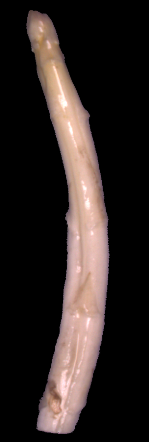
\includegraphics[width=0.15\textwidth]{Figures/chapter03/example_img_bent.png}
  \end{center}
  \vspace{-15pt}
  \caption[Example Image Feature Bent]{ \textbf{Feature Bent}~~~~~~~~}
  \label{fig:ExampleBent}
\end{wrapfigure}

\bigskip
An asparagus is categorized as having the feature bent, if the shape of the asparagus is curved rather than straight (see \autoref{fig:ExampleBent}). 

If it is only slightly curved but can otherwise be thought of as straight -- that means fitting next to other straight spears without standing out -- it is labeled as straight. If the spear looks close to the same on all three pictures regarding its shape, it might indicate that it is heavily bent and therefore cannot be turned on the machine’s conveyor belt.

The feature bent has a broader range of shapes where the asparagus is not obviously deformed but also not completely straight. An exception holds for S-shaped spears, which always count as bent.

\bigskip
In the following, the process for implementing an automatic function for curvature detection is described.
Multiple curvature scores can easily be computed based on regression fits to the centerline of an asparagus spear. For example, the parameters of linear or polynomial regression can be interpreted as a description of how bent an asparagus spear is. 

\bigskip
Deriving sparse descriptions is based on a two-stage approach. In the first stage, the centerline of an asparagus spear is computed because it is considered to be a good description of the curvature of asparagus spears. In each image the asparagus spear is roughly vertically oriented. This means that also for bent spears the head lies within the top center of the image (see \autoref{sec:Preprocessing}). The centerline is computed by binarizing the image into foreground and background and computing the mean of pixel locations along the vertical axis (i.e.\ for each row). The resulting binary representation shows a single pixel line. It serves as the input to the second stage of curvature estimation.

In the second stage, curves are fit to the pixel locations of the centerline. For a simple score, linear regression is employed and the sum of squared errors is thresholded and interpreted as a curvature score. This score is small for perfectly straight asparagus spears and increases the more bent an asparagus is. As an S-shaped asparagus is arguably perceived as bent even when the overall deviations from the center line are small, a second descriptor was computed as the ratio between the error of a linear fit and polynomial regression of degree three. Thresholding values and employing a voting scheme for the results for all three perspectives yields a rule to measure curvature (e.g.\ at least one of the three perspectives indicates that the asparagus is bent). However, it has again proven difficult to set thresholds appropriately to reliably capture the visual impression. Hence, another sparse representation was calculated by dividing the spears into several segments and fitting linear regression to each segment. A \acrfull{mlp} was trained on the resulting 18 angles per asparagus (see~\autoref{subsec:FeatureEngineering}).

\bigskip
Calculating a score for curvature is fast and efficient. While the respective approach is suitable to define curvature on a technical level, it does not necessarily meet up with the subjective perception of how bent an asparagus appears. Just like histograms of palette images, curvature scores are the results of feature engineering: The use of extensive domain knowledge to filter relevant features~\citep{zheng2018feature}. They can serve as an input to a machine learning approach that maps this sparse representation to the target categories (see~\autoref{subsec:FeatureEngineering}).

\begin{wrapfigure}{!I}{0.35\textwidth}
  \begin{center}
    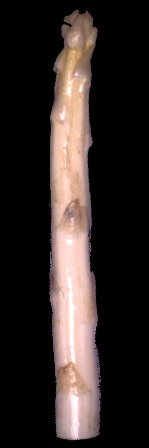
\includegraphics[width=0.15\textwidth]{Figures/chapter03/example_img_flower.png}
  \end{center}
  \vspace{-15pt}
  \caption[Example Image Feature Flower]{ \textbf{Feature Flower}}
  \label{fig:ExampleFlower}
\end{wrapfigure}

\subsubsection{Flower}
\label{subsec:Flower}

An asparagus is graded as having the feature flower when the bud shape of the head is more developed, as in \autoref{fig:ExampleFlower}.

When a bud is in full bloom, it is clearly visible. However, it can be quite difficult to distinguish between an asparagus with clearly cut but closed petals and an asparagus that has just begun to develop a flower. It was decided to label the feature as absent when the asparagus does not clearly show the characteristic flower. With this decision, we aimed to reduce the correspondence error between annotators.

\bigskip
The implementation of the flower detection function turned out to be difficult to realize. Several approaches have been tested, but none of them generated sufficiently good results. Two main notions were tried. The first approach uses the shape of the head as an indicator for a flower. The idea is that asparagus spears with a flowery head exhibit a more open head shape. In other words, the head looks less round and has no smooth outline, but shows fringes. The second approach focuses on the structure within the head. Supposedly, asparagus with flowery heads exhibit more edges and lines in the head area. In both cases, it is challenging to find a way to discriminate between asparagus with and without flowery heads. One reason for that is the poor resolution of the camera that is installed in the sorting machine. With a pixel to millimeter ratio of around four to one\footnote{The ratio was not calculated by us but is an information provided by the manufacturer \citep{autoselectanleitung}.}, it is even difficult to detect flowers with the human eye. Likewise, the current software in the machine struggles greatly with the classification of this feature.

\begin{wrapfigure}{!I}{0.35\textwidth}
  \begin{center}
    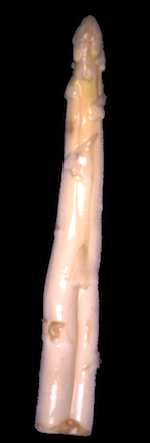
\includegraphics[width=0.15\textwidth]{Figures/chapter03/example_img_hollow.png}
  \end{center}
  \vspace{-15pt}
  \caption[Example Image Feature Hollow]{ \textbf{Feature Hollow}}
  \label{fig:ExampleHollow}
  \vspace{15pt}
\end{wrapfigure}


\subsubsection{Hollow}
\label{subsec:Hollow}

It was not possible for us to implement the feature hollow in an automatic, classical computer vision approach. Thus, only labels from the human annotators are available for this feature.

\bigskip
The feature hollow indicates if the spear has a cavity inside.
This might be expressed by a bulgy center and a line running vertically along the spear’s body. Another, more distinct indicator is an asparagus that looks like two spears fused together (see \autoref{fig:ExampleHollow}). A hollow asparagus can be confused with a very thick asparagus.

The feature hollow can occur without showing a clear line or obvious bulge at its center. Therefore, there is a high risk of wrong classification.The feature can be easily checked when you have physical access to the asparagus. If the asparagus is actually hollow, it will have a hole at its bottom. Unfortunately, this cannot be discovered when only looking at the spears from the side.


\subsubsection{Not classifiable}
\label{subsec:NotClassifiable}

The feature not classifiable is no feature to an asparagus per se. It is therefore not implemented as an automatic feature extraction approach. However, it is integrated into the hand-label application and can be selected by the human annotators if applicable.

That is, whenever the spear is unrecognizable, the head part of the spear is severed, two spears are present in one picture (as in \autoref{fig:ExampleThickness}), the spear is cut off by the image, or other unusual circumstances occurred, it falls into the category of being unclassifiable.


\subsection{The hand-label app: A GUI for labeling asparagus}
\label{sec:LabelApp}

The previous section shows that some features are reliably measurable by means of classical computer vision. This holds especially for simple features such as length and width of an asparagus but to a certain degree also for curvature. In contrast, for features that relate to small details such as the feature flower direct measurements have proven to be difficult (see \autoref{subsec:Flower}). The application of machine learning for measuring these features appears as a promising alternative. 
However, the major part of our dataset consists of unlabeled data. Considering the amount of data that could potentially be labeled, a custom interface is required that allows for a time efficient attribution of labels.


\subsubsection{Motivation}
\label{subsec:Motivation}

An efficient way of manually attributing labels becomes especially important if a very large amount of labeled data is required. Providing a sufficiently large, labeled data set is one of the major non-algorithmic challenges in the application of machine learning for classification tasks~\citep{al2018labeling}. Missing labels are especially problematic if supervised learning methods such as feed forward \acrshortpl{cnn} are employed. Depending on the variance of the data a large number of samples is required~\citep{russakovsky2015imagenet}.

\bigskip
The options to reduce the variance and hence the need to attribute labels to a very large number of samples are limited. We employed preprocessing and manual feature engineering to reduce the variance and tested strategies on the algorithmic domain such as unsupervised and semi-supervised learning as they promise to work with relatively few labels (see \autoref{sec:SemiSupervisedLearning} and  \autoref{subsec:FeatureEngineering}). Nonetheless for training and more importantly performance evaluation of machine learning models a substantial amount of labels are required. Otherwise quality metrics such as accuracies, sensitivity and specificity cannot be calculated. Hence labels had to be manually attributed.

Annotating labels manually requires plenty of effort. \blockquote{Data set annotation and/or labeling is a difficult, confusing and time consuming task} \citep[p.~2]{al2018labeling}. Human performance is often acknowledged as the baseline or \enquote{gold standard}’. Especially for image classification human labeled data is used.\footnote{For example the performance of GoogLeNet is compared to human level performance using the ImageNet data set \citep{russakovsky2015imagenet}.} Considering the amount of data that has to be labeled, a custom interface is required that allows for time efficient attribution of labels.

We decided to attribute labels for each of the previously described features other than the width and the length to at least 10000 asparagus spears (and hence evaluate 30000 images). This means that several ten thousand judgements had to be made which highlights the importance of a tool that allows to make this process as quick as possible.


\subsubsection{The Labeling Application}
\label{subsec:LabelApp}

A custom application was built aiming for a quick and intuitive labeling process.\footnote{ See \url{https://github.com/CogSciUOS/asparagus/tree/FinalProject/labeling/hand\_label\_assistant} (as of 11/27/2020)} Questions appear alongside depictions of an asparagus spear and the user answers them using the designated buttons or keys. Once all questions are answered the next asparagus appears automatically and the procedure is repeated. To assist the users in their judgement some automatically extracted features such as the length or width of the asparagus spear as well as a color histogram are displayed.

\begin{figure}[!htb]
    \centering
    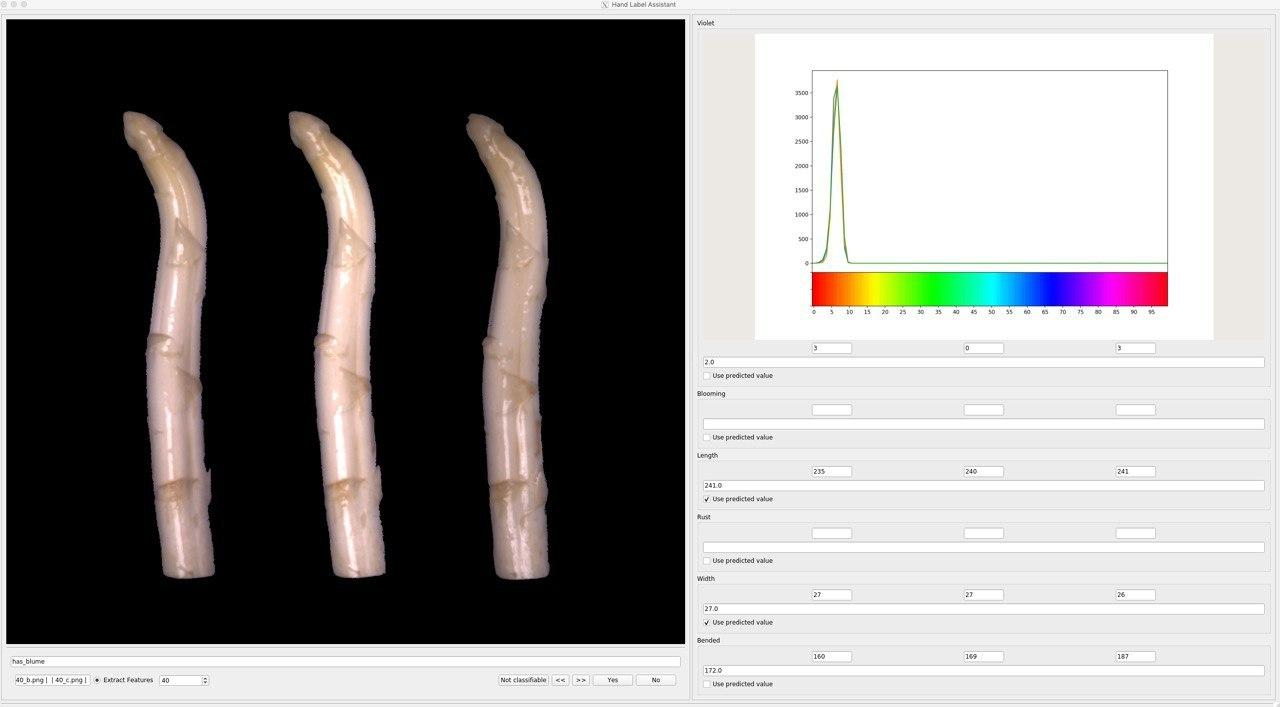
\includegraphics[scale=0.3]{Figures/chapter03/labelapp_example.png}
    \decoRule
    \caption[The Labeling Dialog of the Hand-Label App]{\textbf{The Labeling Dialog of the Hand-Label App}~~~The depiction shows the main dialog used for labeling. In the left part all three available images (perspectives) for the asparagus are shown with the ID 40. The current question that targets at one of the features of interest is displayed in the area below the images. They are phrased such that the user can answer them with yes or no using the respective buttons or keyboard controls. The results  of the automatic feature extraction are displayed on the right side. The upper right panel shows the histogram of color hues.}
    \label{fig:LabelAppGUI}
\end{figure}

The app comprises two user interfaces: A startup window that allows for a preview of asparagus images and the attributed labels (represented by Ui\textunderscore Asparator) and the main labeling interface (Ui\textunderscore LabelDialog) (see \autoref{fig:LabelAppDiagram}). Using the labeling interface is possible only after the user selects the source folder of images and specifies or loads a file that contains the attributed labels. This ensures that the file paths for input and output are set. A dictionary that maps indices to images can be parsed from file names and the minimum index is determined. As such, the label dialog and the respective controller class always reside in a valid initial state. For labeling, the user answers questions that are displayed alongside the images. The result is saved and the next question will automatically appear upon answering.

Automatic feature detection can be selected as an alternative for manual labeling for specific features. The result is displayed and saved to a file. This flexible approach was chosen as it was initially unclear and disputed in how far automatic feature extraction yields satisfying results. Further, it allowed to improve automatic feature extraction methods and to develop an intuition for the characteristics of the features. On top of that, it has been proven to be useful for debugging.

\bigskip
The development of the app was accompanied by three major challenges. First, handling a large data set of several hundred gigabytes that is accessible in a network drive. Second, changing requirements that resulted from group decisions. This required substantial changes of the initial architecture and the reimplementation of parts of the code. The third challenge is related to the question of the handling of internal states of the app. 
Internal states of the app are handled such that it is possible for the user to navigate into states for which no images are available. All cascades of methods of the app including preprocessing functions that require the respective images as an input are adjusted such that they can handle this case. The architecture is beneficial as it allows the user to manually iterate over asparagus IDs without being interrupted because an ID relates to an invalid or missing file. It was chosen over alternatives to handle invalid states as it was considered the easiest to implement and meets requirements given by the PyQt framework.

\begin{figure}[!t]
    \centering
    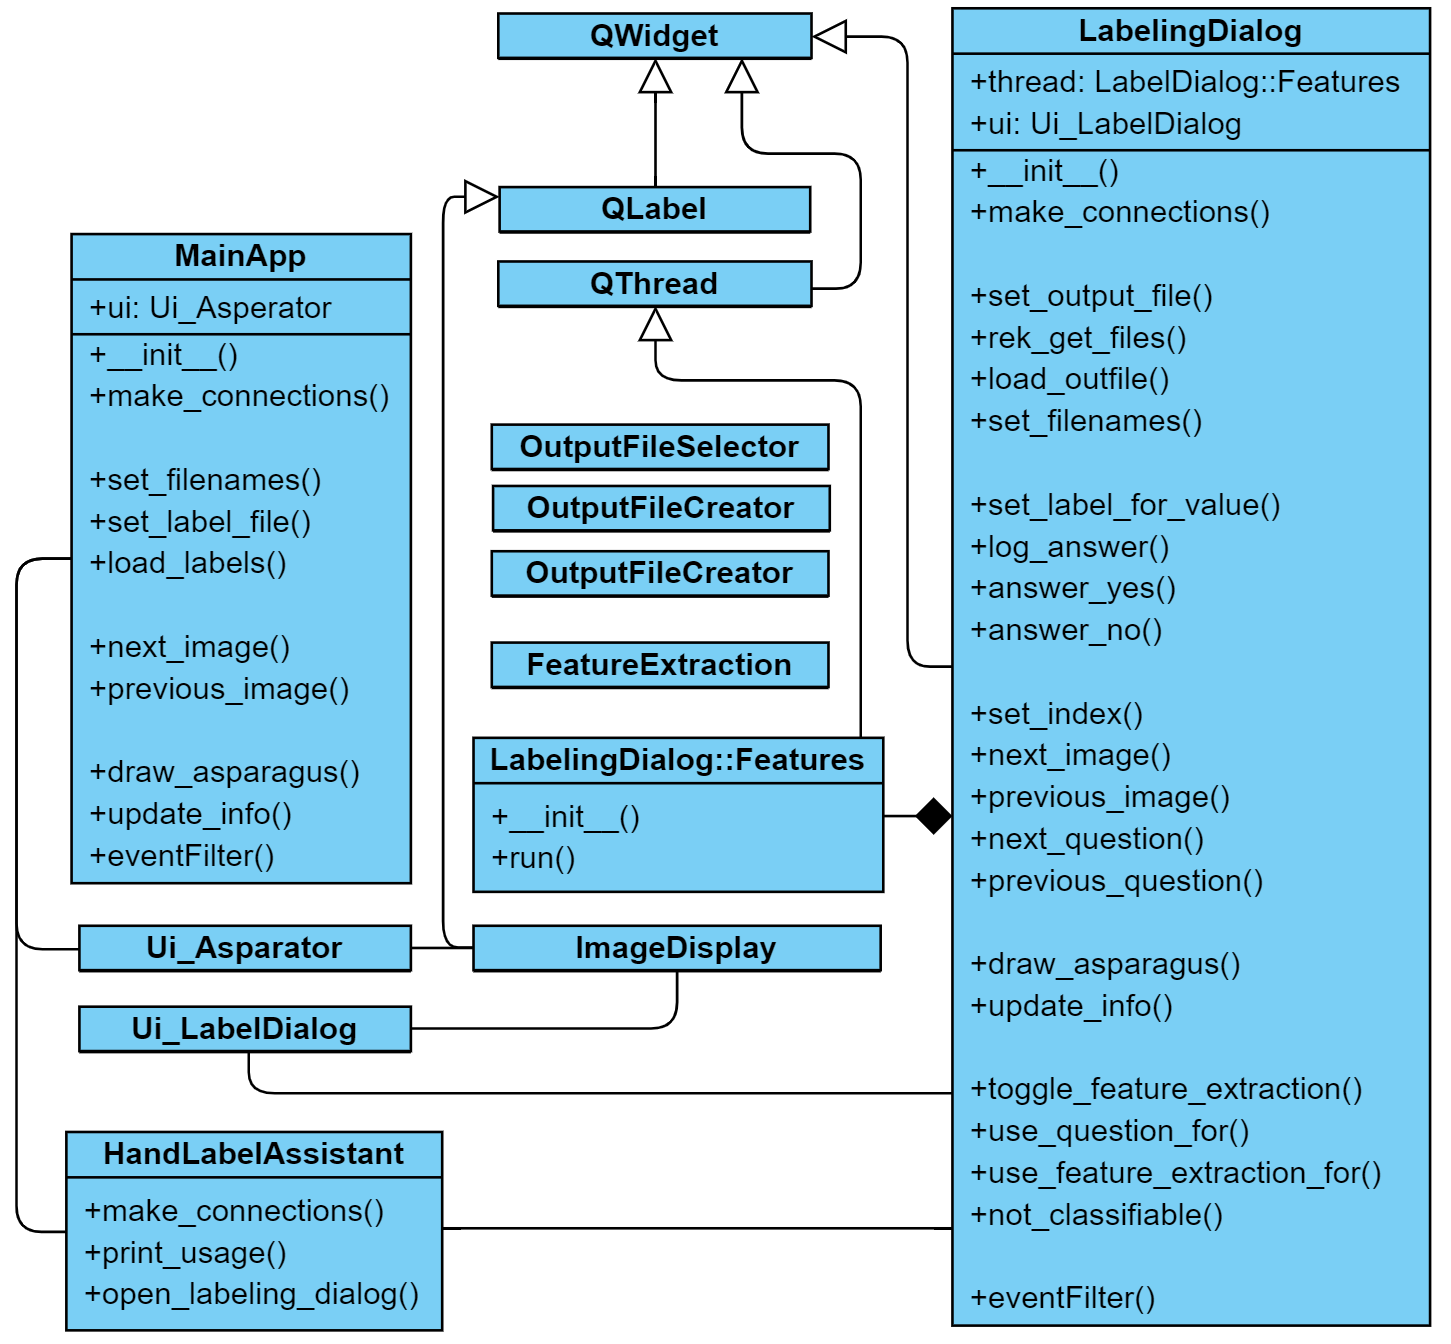
\includegraphics[scale=0.3]{Figures/chapter03/label_app_diagram.png}
    \decoRule
    \caption[UML Diagram for the Hand-Label App]{\textbf{UML Diagram for the Hand-Label App}~~~The depiction shows the class diagram for the hand-label app in \acrshort{uml}.}
    \label{fig:LabelAppDiagram}
\end{figure}

The app is implemented using the PyQt5 framework\footnote{see \url{https://pypi.org/project/PyQt5/} (visited on 04/24/2020)} while coarsely following the model, view controller principle. Model and controller are not strictly separated and thus no distinct model class or database is used. Instead the labels are managed as a Pandas DataFrame and serialized as a csv-file. Upon state change (i.e.\ index increment), images are loaded from the network drive that is mounted on the level of the operating system. The views are designed using QtDesigner. Controller classes, utility classes for feature extraction (Features) and a custom ImageDisplay were manually implemented.  \autoref{fig:LabelAppDiagram} shows the \acrshort{uml} class diagram.


\subsection{Manual labeling}
\label{sec:ManualLabeling}

In this section, the process and the results of manually labeling the data with the help of the hand-label app is laid out. The labeling criteria which allocate each spear to a single quality class were explained in the subsections of the section \nameref{sec:AutomaticFeatureExtraction}. The outcome of the labeling process and one approach to measure the agreement of the manual labeling will be described in the following subsections.

\begin{figure}[!htb]
	\centering
	\vspace{20pt}
	\begin{subfigure}{0.3\textwidth}
		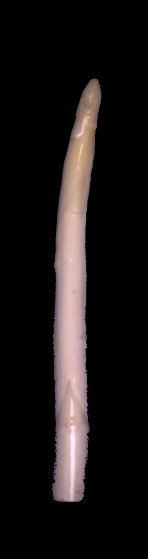
\includegraphics[width=0.80\linewidth]{Figures/chapter03/diff-img-bent.png}
		\caption{bent?}
	\end{subfigure}
	\begin{subfigure}{0.3\textwidth}
		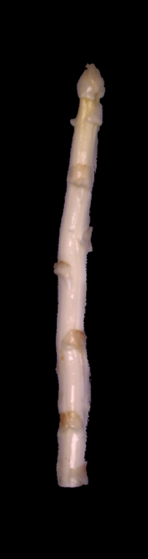
\includegraphics[width=0.80\linewidth]{Figures/chapter03/diff-img-flower-rust.png}
		\caption{flower?}
	\end{subfigure}
	\begin{subfigure}{0.3\textwidth}
		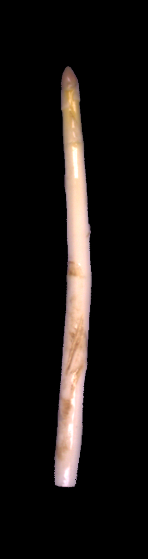
\includegraphics[width=0.80\linewidth]{Figures/chapter03/diff-img-violet.png}
		\caption{violet?}
	\end{subfigure}
    \caption[Examples of Critical Images]{\textbf{Examples of Critical Images}~~~Three examples of asparagus are shown where the corresponding feature label is difficult to determine -- thus, a critical decision has to be made. Image (A) displays an asparagus that shows a slight S-curve, however, not very strong. It might be labeled as being bent or as not being bent by the annotator. Images (B) and (C) show asparagus with brown spots which can be judged either as rust or as pressure marks (no rust), again depending on the annotator. Additionally, it is not obvious whether the asparagus in (B) exhibits a flower or whether the spear in (C) is of violet color at the head region.}
    \label{fig:CriticalExampleImages}
\end{figure}

\bigskip
The images were labeled for their features by all members of the group with the hand-label app (described in \autoref{sec:LabelApp}). As none of the team members were experts in asparagus labeling, a general guideline for the feature labeling had to be established (see \autoref{sec:AutomaticFeatureExtraction}). The guideline was written in accordance with the owner of the asparagus farm Gut Holsterfeld, Mr. Silvan Schulze-Weddige. He was consulted in all questions regarding the labeling of the asparagus.

General challenges in the manual labeling in front of a computer screen, including the respective image quality and the variance in the agreement of the project members, were expected from the start. As the task relies on the subjective view of individual humans, opinions about the presence or absence of features can diverge. By consulting Mr. Schulze-Weddige on difficult cases, it became clear that even for experts some examples are difficult to classify from image data (see \autoref{fig:CriticalExampleImages}).

To tackle the issue and to have an overview of the general agreement of the labeling between group members, a measure was applied, namely the Kappa Agreement. The Kappa Agreement is used to assess the degree of accordance in labeling between the single members and to monitor how the labeling agreement developed during the manual labeling process. 


\subsubsection{Labeling outcome}
\label{subsec:SortingOutcome}

In this section, the process and the results of the labeling with the hand-label app are described.

\begin{figure}[!ht]
	\centering
	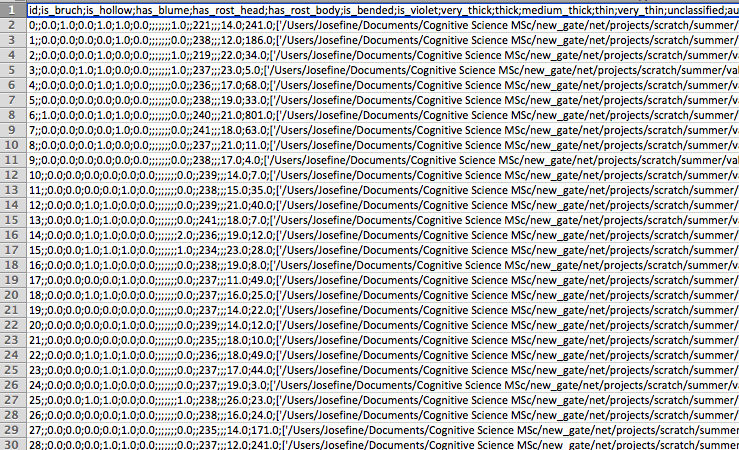
\includegraphics[scale=0.5]{Figures/chapter03/csv_overview.png}
	\decoRule
	\caption[Manual Labeling Output CSV-File]{\textbf{Label File}~~~The feature labels extracted by the manual labeling process are saved in a csv file. This image shows the beginning of the file \texttt{combined\textunderscore new.csv} in which all label files were later combined as one.}
	\label{fig:CSVfileOverview}
\end{figure}

The labels of all labeled images are stored in a csv-file, as shown in~\autoref{fig:CSVfileOverview}. The first entry is the image identification number. Every feature can be of value 0, value 1 or empty. Whenever a feature is present in an image, the value is set to 1. If the feature is absent, it is set to 0. For images labeled as not classifiable, all feature values remain empty. The image path to every of the three images for one spear is also saved in the label file in a separate column. After the labeling process, the individual csv-files with the labels are merged into one large \texttt{combined\textunderscore new.csv} file. The content of this file is later used for the classification of the data with the different approaches (see \autoref{ch:Classification}). It can be found in the study project’s GitHub repository.\footnote{~See \url{https://github.com/CogSciUOS/asparagus/tree/FinalProject/preprocessing/get_data} (as of 11/27/2020)}

\begin{table}[!hb]
	\centering
	\vspace{10pt}
	\resizebox{.75\linewidth}{!} & \textbf{Feature} & \textbf{\%} \\
		\hline
		hollow		&  3.3\%		& fractured			& 3.5\% 		\\
		flower		& 12.9\% 	& very thick 		& 4.0\% 		\\
		rusty body	& 45.5\% 	& thick 				& 29.1\%	 	\\
		rusty head~~~~~~~~~~~~~~~~~~& 14.7\% & medium thick & 18.7\% 	\\
		bent 		& 40.0\% 	& thin				& 17.9\% 	\\
		violet 		&  7.9\% 	& very thin 			& 30.3\% 	\\
		{} 	 		& {}  		& not classifiable~~~~~~~~~~~~~~& 2.1\%		\\
		\hline
	\end{tabular}%
	}
	\caption[Manual Labeling Feature Representation]{\textbf{Feature Representation in the Data Set} \\ In this table, the representation of each feature in the manually labeled 13319 asparagus samples is reported in \%.}
	\label{tab:FeatureRepresentation}
\end{table}

\bigskip
The manual labeling took place over the period of November 2019 to January 2020. A session usually consisted of 500 images. A session of labeling 500 images took between two and four hours. The average time spent for labeling one asparagus is around 27 -- 48 seconds.

All in all, 13319 triples of images were labeled for their features. There is a large variance in the presence of the features in the data as shown in~\autoref{tab:FeatureRepresentation}. Of the acquired 13319 images, the feature most present in the data is rusty body with 45.5\%, followed by the feature bent with 40\%. Features whose representation is below 10\% include the features violet (7.9\%), hollow (3.3\%), fractured (3.5\%), and very thick (4\%). The feature not classifiable shows least presence with 2.1\%.

It emerges that many features are only sparsely present in the data. This poses an imbalance in the data that is relevant for later classification tasks and the usage of the data set.

Further, every member of the group participated in the labeling but not everybody labeled the same amount of images. Due to this circumstance, the labeling bias of certain members is more present in the data than of others.

The manual labeling was stopped when the amount of classified data exceeded 13000 samples. We had reached our time limit for labeling samples and needed to begin with training our classification approaches.\footnote{To get an intuition of how much labeled data we might need, we found some of the suggestions in a blogpost helpful which can be visited at \url{https://machinelearningmastery.com/much-training-data-required-machine-learning/} (visited on 04/29/2020). However, we did not find an exact number when to stop labeling.}


\subsubsection{Agreement Measures}
\label{subsec:AgreementMeasures}

When different annotators label data, it is indispensable to verify the degree of agreement among raters. In order to judge how consistently the data is labeled, several statistical methods (inter-rater-reliability) can be applied.

\bigskip
For the current purpose, different agreement measures, all implemented by scikit-learn, are used. The first is Cohen’s Kappa. It is seen as a more robust measure than a simple agreement percentage, such as a measure of true positives and true negatives, which was traditionally used for those cases~\citep{cohen1960coefficient}. Cohen’s Kappa is more robust, as the rate of agreement occurring by chance is included in the calculation. This method is applicable to compare the rating of two raters on a classification problem. The degree of agreement is always within $-1.0$ and 1.0 inclusive. The greater the Kappa value, the higher the agreement. Values around zero indicate no agreement and negative values indicate negative agreement which can be interpreted as systematic disagreement. Values between 0.41 -- 0.6 are seen as moderate agreement, 0.61 -- 0.8 as substantial agreement, and everything above as almost perfect agreement. All scores below 0.4 are interpreted as unacceptable \citep{mchugh2012interrater}.

Another statistical method used to measure our agreement is the F1 score. The F1 score is used for the evaluation of binary classification. It relies on both precision as well as recall of a test. An F1 score value lies between 0.0 and 1.0 -- the greater the F1 score, the higher the agreement.

Lastly, we calculated the accuracy measure. For a normalized accuracy score, the values lie between 0.0 and 1.0, and the best performance is 1.0. This measure returns the fraction of correctly classified samples. It is a less robust measure than Cohen’s Kappa score~\citep{mchugh2012interrater}.


\subsubsection{Reliability}
\label{subsec:Reliability}

In order to evaluate the degree of agreement of our data, we measured the agreement at two different points in time.\footnote{for our API documentation see \url{https://asparagus.readthedocs.io/en/latest/api/measure\textunderscore agreement.html} (as of 11/27/2020)}

First, six annotators assigned feature labels to images out of each class of the pre-sorted asparagus that we obtained by running the spears through the machine twice. We ensured that two different annotators labeled the same set of images. The Kappa scores varied strongly between annotator pairs and features from $-0.03$ to 0.76, while the accuracy scores ranged from 0.49 to 1. We were surprised that the agreement scores are low, even though the raters gave the same label to many of the asparagus spears. This is an acknowledged problem~\citep{powers2012problem,sim2005kappa,feinstein1990high,posterFlight}.

\begin{figure}[!ht]
    \centering
    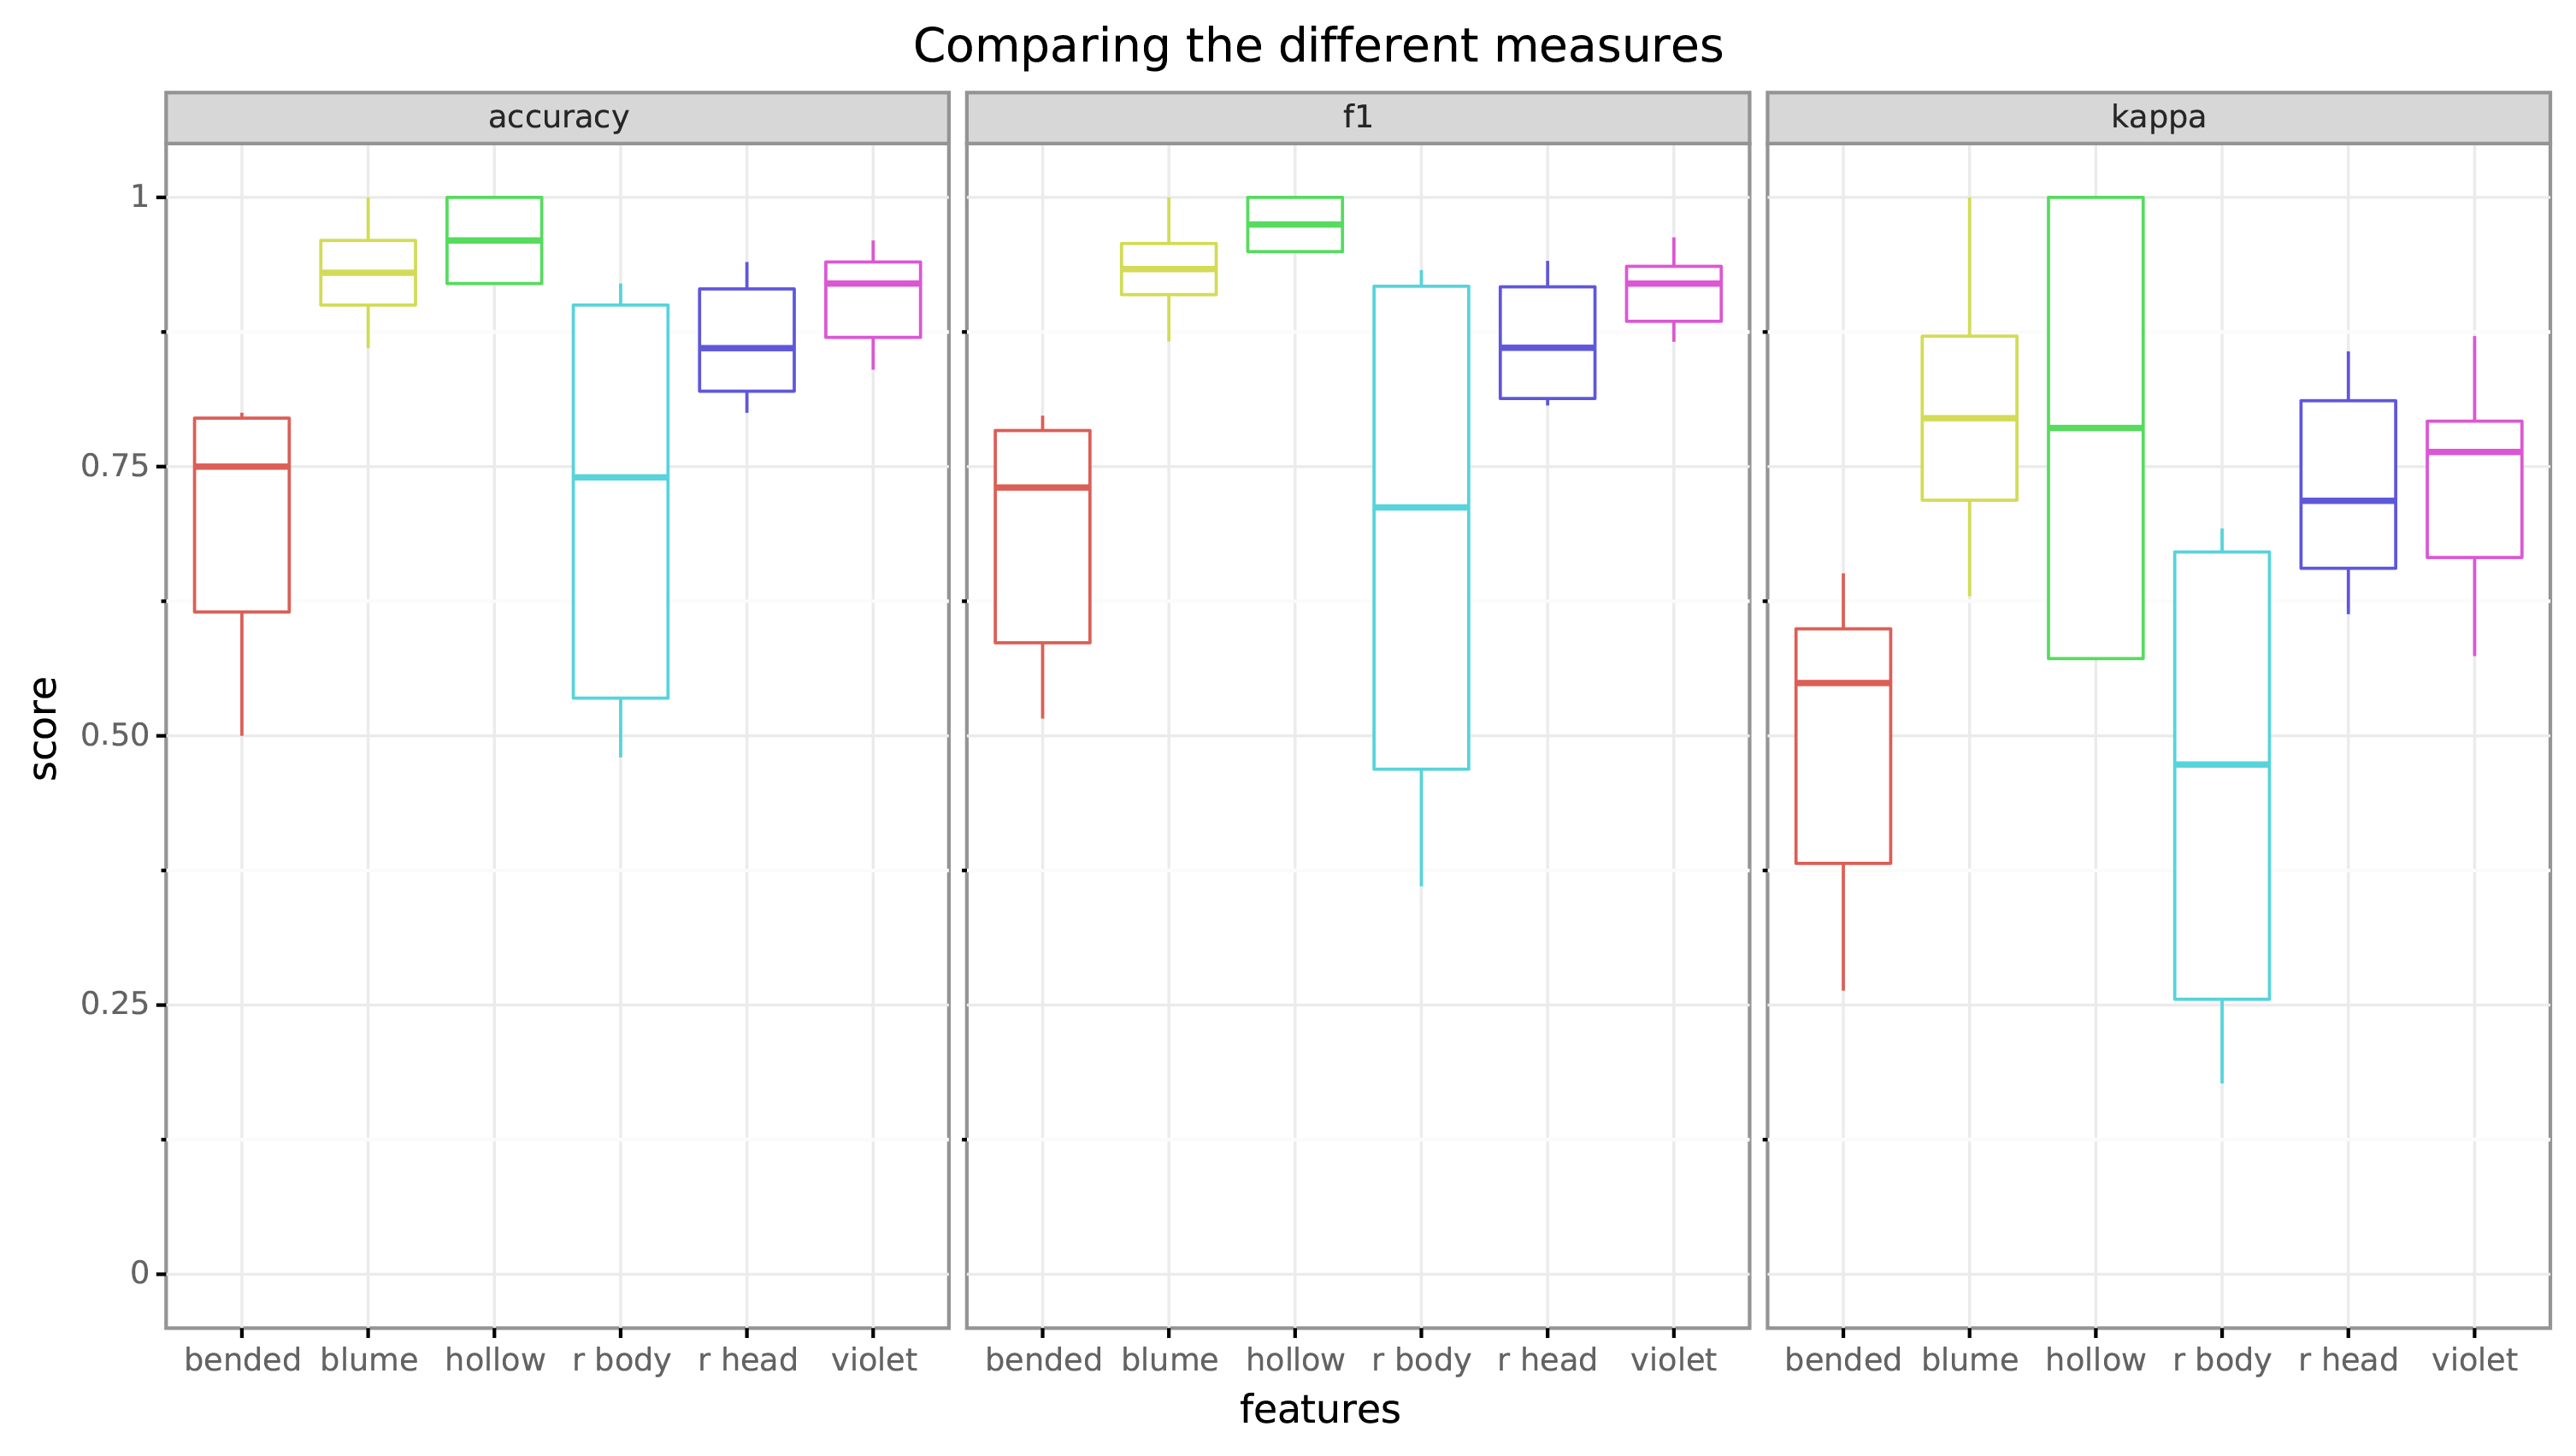
\includegraphics[scale=0.55]{Figures/chapter03/kappa_measurewise.png}
    \decoRule
    \caption[Agreement Measure-Wise Comparison of all Features]{\textbf{Comparing Measures}~~~The figure shows the agreement measures accuracy, F1 and Cohen’s Kappa, separately for each manually labelled feature. Shown are the box-plots, so the middle line indicates the median, the box indicates the IQR. All scores are aggregated scores over all annotator pairs.}
    \label{fig:KappaMeasurewise}
\end{figure}

\begin{figure}[!ht]
    \centering
    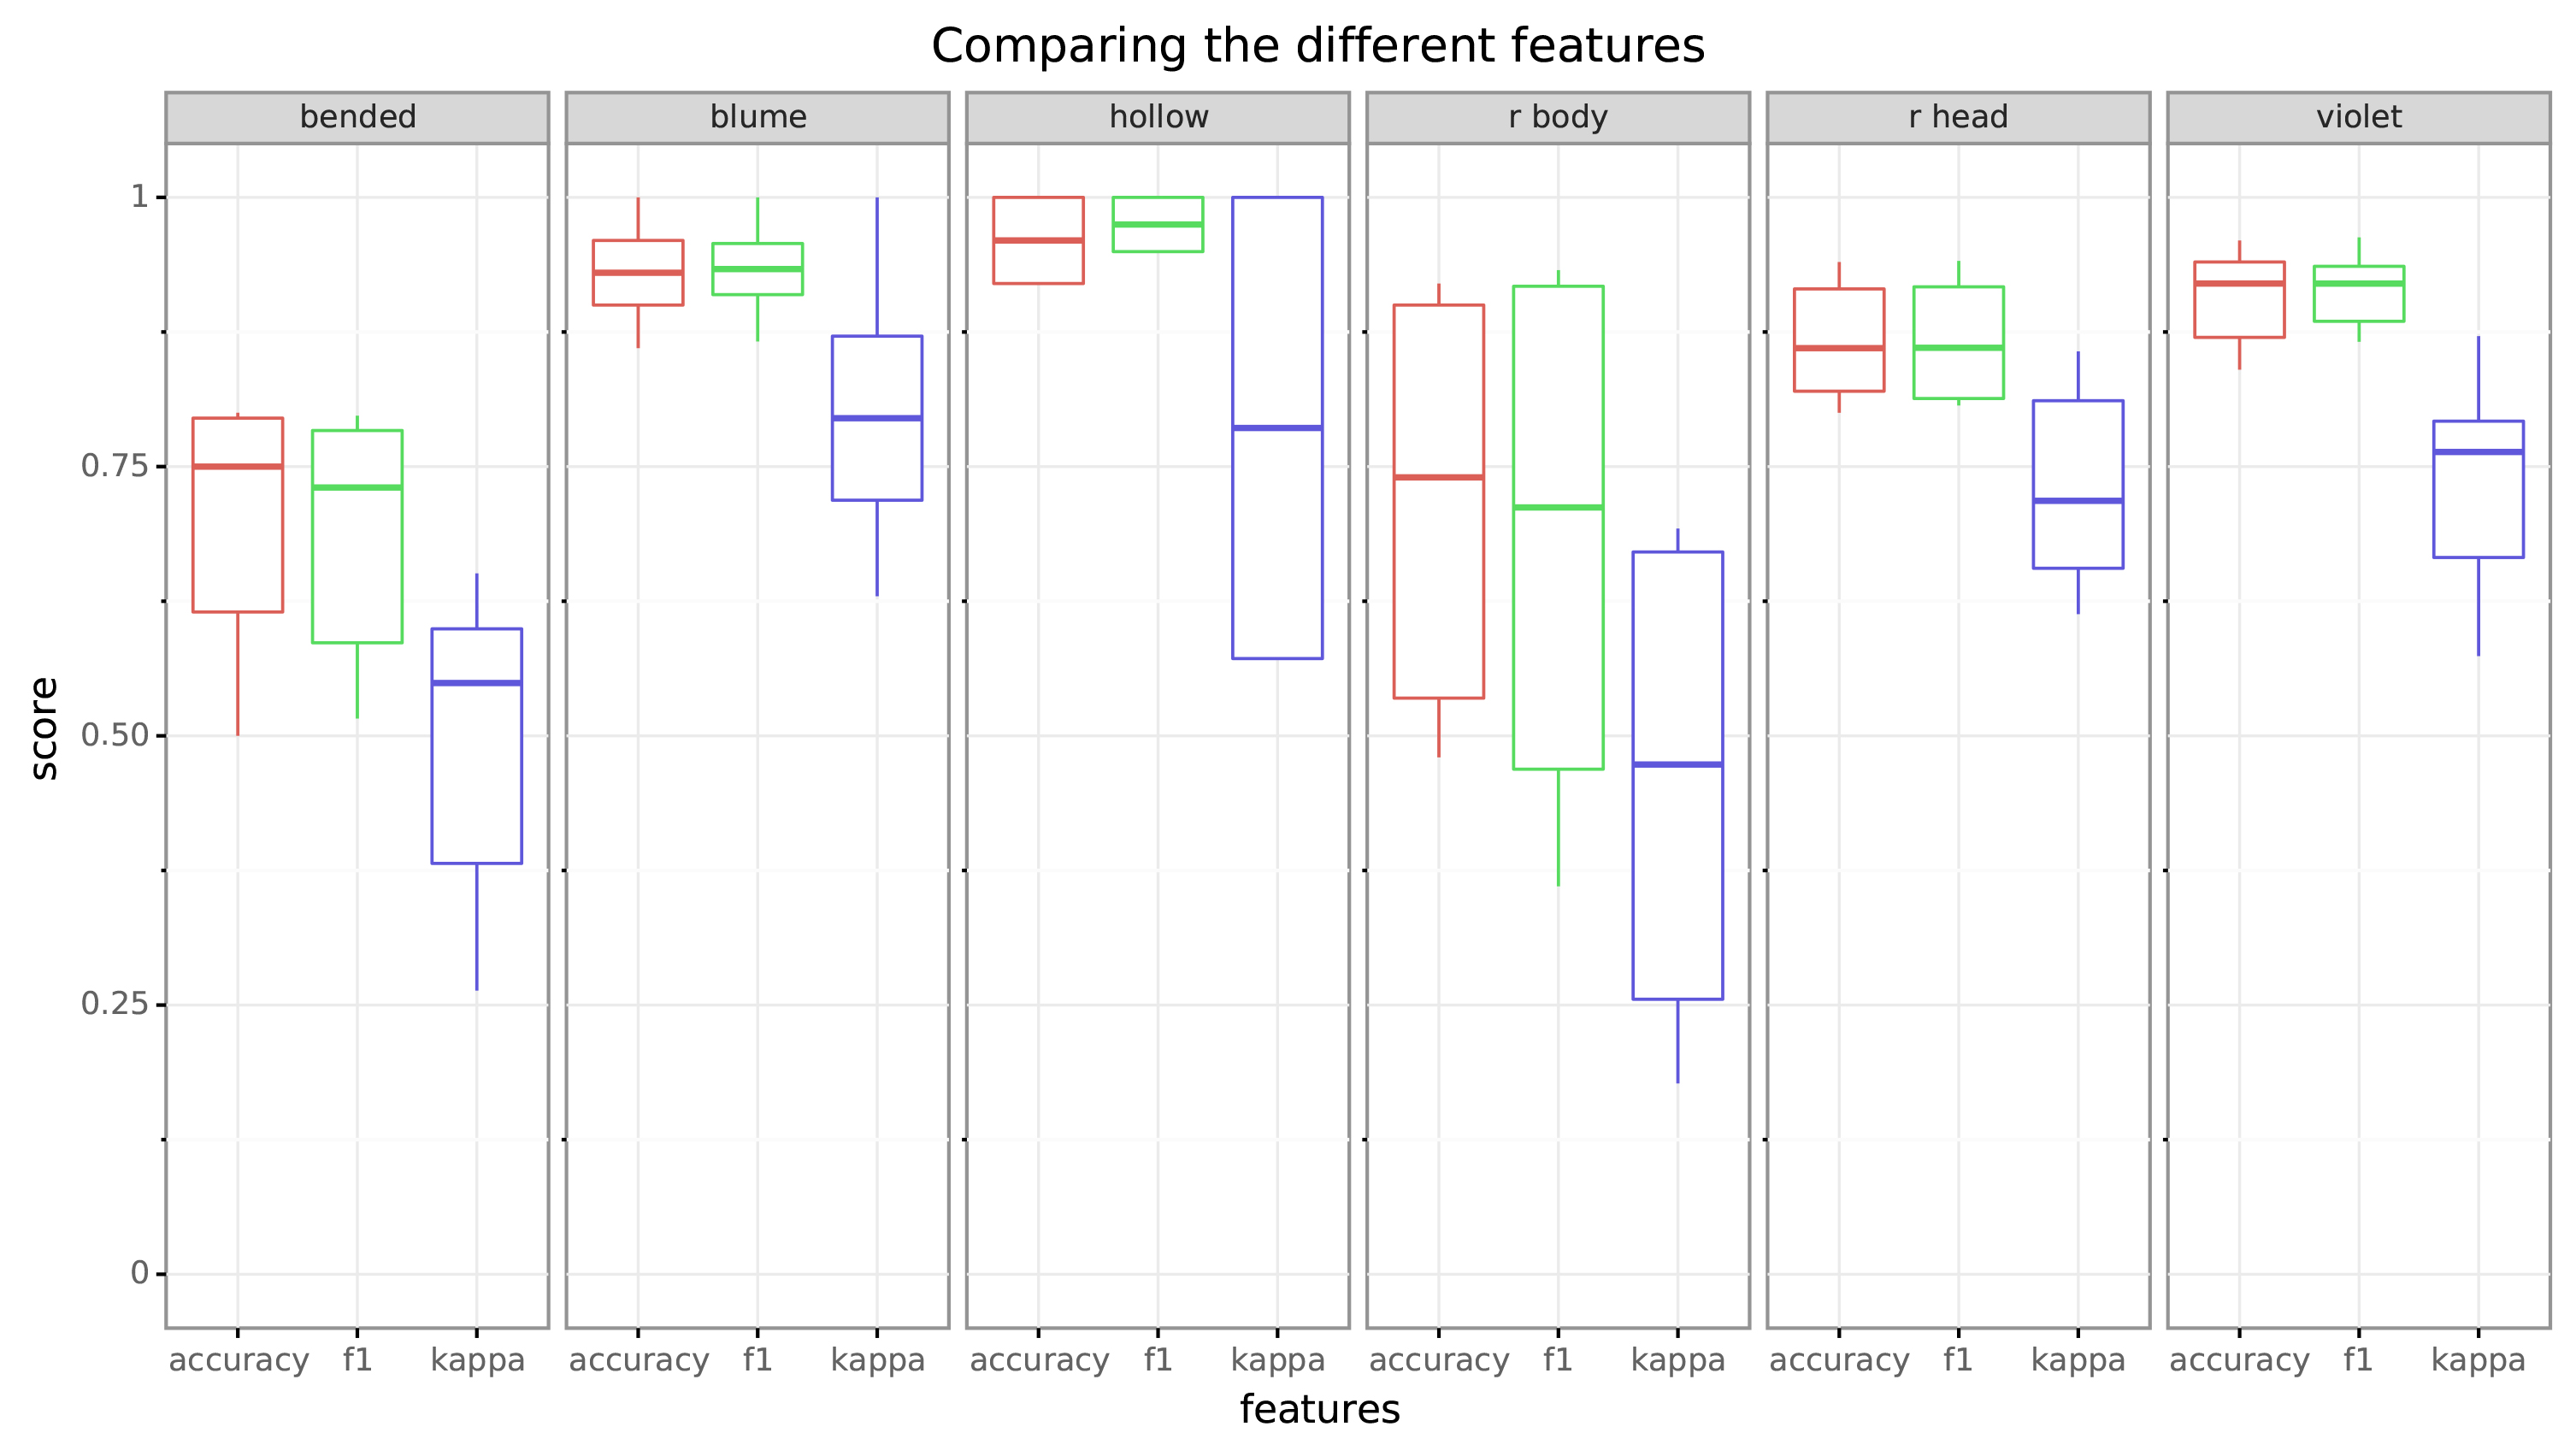
\includegraphics[scale=0.55]{Figures/chapter03/kappa_featurewise.png}
    \decoRule
    \caption[Feature-Wise Comparison of Agreement Measure Scores]{\textbf{Comparing Features}~~~The figure shows each feature separately. For each feature, the corresponding accuracy, F1 and Cohen’s Kappa score is given. Shown are the box-plots, so the middle line indicates the median, the box indicates the IQR. All scores are aggregated scores over all annotator pairs.}
    \label{fig:KappaFeaturewise}
\end{figure}

A reason for the variance in our results could be that we compared the agreement class-wise. Thus, the occurrence of 1s and 0s per class is very unbalanced (for example the class I~A~Anna has very few 1s because the binary features rusty head, rusty body, hollow, bent and violet are not present in this class label). For Kappa scores, if the distribution of 0s and 1s is not balanced, disagreement of the underrepresented value is punished more heavily.\footnote{see also \url{https://stats.stackexchange.com/questions/47973/strange-values-of-cohens-kappa} (visited on 04/24/2020)} Therefore, we decided to repeat the agreement measure feature-wise on non-labeled images, so that the annotators cannot anticipate a specific class label. In order to better understand the reliability of our data, we additionally decided to look at the accuracy score and the F1 score. Beforehand, the team labeled another 50 images all together, clarified classification boundaries again and discussed unclear images (see \autoref{fig:CriticalExampleImages}).

The second time, 50 images were labeled by four annotators. The agreements were measured annotator-pair-wise, and then averaged. The results in the Cohen’s Kappa score vary between features, and annotator pairs. The highest aggregated kappa score over all annotator pairs is reached for the features flower (0.79) and hollow (0.79), then violet (0.76), rusty head (0.72), bent (0.55) and lastly for rusty body (0.47).
For the features flower, rusty head and violet, the interquartile range (IQR) is quite small, whereas the IQR for hollow, bent and rusty body is much larger (see \autoref{fig:KappaMeasurewise} and \autoref{fig:KappaFeaturewise}).

The agreement scores accuracy and F1 yield very similar results. Results are slightly better than the Kappa scores, in total and for each feature. The highest median accuracy score is reached for the feature hollow (0.96), then flower (0.93), then violet (0.92), then rusty head (0.86), then bent (0.75) and then rusty body (0.74). The order is the same for the F1 scores. The median F1 scores lie between (0.71 and 0.97).

\bigskip
All in all, it can be said that the agreement scores indicate moderate up to substantial agreement. Regardless of the measurement, agreement is highest for the features flower, violet and rusty head.


\subsection{The asparagus data set}
\label{sec:AsparagusDataSet}

In the following chapter, the asparagus data sets will be discussed. The data that we collected is restructured and preprocessed into several different versions which are used for the classification approaches. Further, the possibility to save a the dataset as Tensor with the numpy API or as serialized \texttt{TFRecord} files with the \mbox{\texttt{tf.data.dataset}} API are introduced. These methods are compared and followed by a recommendation for further work with the data set.

One peculiarity about our data is its variance. The differences in the features which decide the class label of an asparagus are very small. Overall, asparagus spears look very similar. This differentiates our classification task from other examples in the literature which usually have a high inter-class difference.To facilitate the learning process and help the model focus on the most important information, we removed irrelevant differences (eg. in the background) from the images. (see Chapter ~\ref{sec:Preprocessing}).

\subsubsection{Description of our data set(s)}
\label{subsec:DifferentDataSets}


With the help of the preprocessing as described in ~\ref{sec:Preprocessing}~\nameref{sec:Preprocessing}, the raw images are transformed and distributed into different folders which serve as input for the approaches.
The images in the different folders can be distinguished in three ways: the images either have the original background or the background is removed, the asparagus spears are centered and rotated upwards or not and the images are down sampled to reduce memory consumption or in the original resolution.

One data set is constructed with all the labeled images in a single numpy array, which can be stored and loaded at once. As the three perspectives of each asparagus spear are concatenated horizontally, they appear to lie next to each other in the resulting image. These concatenated images are then combined to the final file. The first out of four dimensions in this file depicts the number of labeled asparagus spears. The second and third dimension represent the height and the width of the images, respectively. Further, the fourth dimension represents the three RGB values.
In addition, the images are downscaled to facilitate the training process and reduce memory consumption. Each image is downsampled by a factor of six, that means every 6th pixel is used in the reduced image. This factor can be easily changed to create a new data set.

An additional data set is generated which contains images of the head region of the asparagus spears exclusively. This data set was used to train a dedicated network for head related features (see~\autoref{subsec:HeadNetwork}).


\subsubsection{Data set creation with Tensorflow}
\label{subsec:DataSetTheory}

As pointed out before more than 800 Gigabyte (GB) of preprocessed image data was generated. This big amount of data for training and evaluation in different approaches was challenging. The main difficulty was memory management, an acceptable training time and data organisation. Especially the size and format of the image has a significant impact on our import pipeline and, therefore, on the total training time. 

In respect to the importance of preventing any loss of information the \texttt{TFRecord} storage format was chosen to retain the data set. Two data sets are created in this file format. One with all files that were preprocessed with a size of 225 GB, and another one with the preprocessed and labeled data, respectively smaller. 

A detailed description of the benefits of the used data format can be found in the appendix at \autoref{subsec:BenefitsDataSet}. In summary, there are advantages using \texttt{tf.data}. On the one hand, it is possible to reduce the disk space and to read the image data faster due to an iterator with parallel and sequential access to the data. On the other hand, many functional transformations to adjust the images with custom preprocessing steps according to the approach can be used in the pipeline, as we did manually.

\bigskip
We tried to add our data set to the \texttt{\acrshort{tfds}} \footnote{See~\url{https://www.tensorflow.org/datasets/beam\_datasets} (visited on 04/26/2020)}. \texttt{\acrshort{tfds}} enables all tensorflow users to access the data set directly using the TensorFlow API. However, the process of publishing the data set turned out to be too time consuming because of the large amount of images. In order to use the benefits of the \mbox{\texttt{tf.data}} API we should have integrated it into our pipeline at an earlier stage.